%% bare_conf.tex
%% V1.4a
%% 2014/09/17
%% by Michael Shell
%% See:
%% http://www.michaelshell.org/
%% for current contact information.
%%
%% This is a skeleton file demonstrating the use of IEEEtran.cls
%% (requires IEEEtran.cls version 1.8a or later) with an IEEE
%% conference paper.
%%
%% Support sites:
%% http://www.michaelshell.org/tex/ieeetran/
%% http://www.ctan.org/tex-archive/macros/latex/contrib/IEEEtran/
%% and
%% http://www.ieee.org/

%% *************************************************************************
%% Legal Notice:
%% This code is offered as-is without any warranty either expressed or
%% implied; without even the implied warranty of MERCHANTABILITY or
%% FITNESS FOR A PARTICULAR PURPOSE!
%% User assumes all risk.
%% In no event shall IEEE or any contributor to this code be liable for
%% any damages or losses, including, but not limited to, incidental,
%% consequential, or any other damages, resulting from the use or misuse
%% of any information contained here.
%%
%% All comments are the opinions of their respective authors and are not
%% necessarily endorsed by the IEEE.
%%
%% This work is distributed under the LaTeX Project Public License (LPPL)
%% ( http://www.latex-project.org/ ) version 1.3, and may be freely used,
%% distributed and modified. A copy of the LPPL, version 1.3, is included
%% in the base LaTeX documentation of all distributions of LaTeX released
%% 2003/12/01 or later.
%% Retain all contribution notices and credits.
%% ** Modified files should be clearly indicated as such, including  **
%% ** renaming them and changing author support contact information. **
%%
%% File list of work: IEEEtran.cls, IEEEtran_HOWTO.pdf, bare_adv.tex,
%% bare_conf.tex, bare_jrnl.tex, bare_conf_compsoc.tex,
%% bare_jrnl_compsoc.tex, bare_jrnl_transmag.tex
%% *************************************************************************


% *** Authors should verify (and, if needed, correct) their LaTeX system  ***
% *** with the testflow diagnostic prior to trusting their LaTeX platform ***
% *** with production work. IEEE's font choices and paper sizes can       ***
% *** trigger bugs that do not appear when using other class files.       ***                          ***
% The testflow support page is at:
% http://www.michaelshell.org/tex/testflow/



\documentclass[conference]{IEEEtran}
% Some Computer Society conferences also require the compsoc mode option,
% but others use the standard conference format.
%
% If IEEEtran.cls has not been installed into the LaTeX system files,
% manually specify the path to it like:
% \documentclass[conference]{../sty/IEEEtran}





% Some very useful LaTeX packages include:
% (uncomment the ones you want to load)


% *** MISC UTILITY PACKAGES ***
%
% \usepackage{ifpdf}
% Heiko Oberdiek's ifpdf.sty is very useful if you need conditional
% compilation based on whether the output is pdf or dvi.
% usage:
% \ifpdf
%   % pdf code
% \else
%   % dvi code
% \fi
% The latest version of ifpdf.sty can be obtained from:
% http://www.ctan.org/tex-archive/macros/latex/contrib/oberdiek/
% Also, note that IEEEtran.cls V1.7 and later provides a builtin
% \ifCLASSINFOpdf conditional that works the same way.
% When switching from latex to pdflatex and vice-versa, the compiler may
% have to be run twice to clear warning/error messages.






% *** CITATION PACKAGES ***
%
% \usepackage{cite}
% cite.sty was written by Donald Arseneau
% V1.6 and later of IEEEtran pre-defines the format of the cite.sty package
% \cite{} output to follow that of IEEE. Loading the cite package will
% result in citation numbers being automatically sorted and properly
% "compressed/ranged". e.g., [1], [9], [2], [7], [5], [6] without using
% cite.sty will become [1], [2], [5]--[7], [9] using cite.sty. cite.sty's
% \cite will automatically add leading space, if needed. Use cite.sty's
% noadjust option (cite.sty V3.8 and later) if you want to turn this off
% such as if a citation ever needs to be enclosed in parenthesis.
% cite.sty is already installed on most LaTeX systems. Be sure and use
% version 5.0 (2009-03-20) and later if using hyperref.sty.
% The latest version can be obtained at:
% http://www.ctan.org/tex-archive/macros/latex/contrib/cite/
% The documentation is contained in the cite.sty file itself.






% *** GRAPHICS RELATED PACKAGES ***
%
\ifCLASSINFOpdf
\usepackage[pdftex]{graphicx}
% declare the path(s) where your graphic files are
\graphicspath{{./}}
% and their extensions so you won't have to specify these with
% every instance of \includegraphics
\DeclareGraphicsExtensions{.pdf,.jpeg,.png}
\else
% or other class option (dvipsone, dvipdf, if not using dvips). graphicx
% will default to the driver specified in the system graphics.cfg if no
% driver is specified.
% \usepackage[dvips]{graphicx}
% declare the path(s) where your graphic files are
% \graphicspath{{../eps/}}
% and their extensions so you won't have to specify these with
% every instance of \includegraphics
% \DeclareGraphicsExtensions{.eps}
\fi
% graphicx was written by David Carlisle and Sebastian Rahtz. It is
% required if you want graphics, photos, etc. graphicx.sty is already
% installed on most LaTeX systems. The latest version and documentation
% can be obtained at:
% http://www.ctan.org/tex-archive/macros/latex/required/graphics/
% Another good source of documentation is "Using Imported Graphics in
% LaTeX2e" by Keith Reckdahl which can be found at:
% http://www.ctan.org/tex-archive/info/epslatex/
%
% latex, and pdflatex in dvi mode, support graphics in encapsulated
% postscript (.eps) format. pdflatex in pdf mode supports graphics
% in .pdf, .jpeg, .png and .mps (metapost) formats. Users should ensure
% that all non-photo figures use a vector format (.eps, .pdf, .mps) and
% not a bitmapped formats (.jpeg, .png). IEEE frowns on bitmapped formats
% which can result in "jaggedy"/blurry rendering of lines and letters as
% well as large increases in file sizes.
%
% You can find documentation about the pdfTeX application at:
% http://www.tug.org/applications/pdftex


% Plotting packages
\usepackage{tikz}
\usetikzlibrary{shapes.geometric, arrows}
\usepackage{pgfplots}
\pgfplotsset{compat=newest}

% *** MATH PACKAGES ***
%
% \usepackage[cmex10]{amsmath}
\usepackage{amssymb}
% A popular package from the American Mathematical Society that provides
% many useful and powerful commands for dealing with mathematics. If using
% it, be sure to load this package with the cmex10 option to ensure that
% only type 1 fonts will utilized at all point sizes. Without this option,
% it is possible that some math symbols, particularly those within
% footnotes, will be rendered in bitmap form which will result in a
% document that can not be IEEE Xplore compliant!
%
% Also, note that the amsmath package sets \interdisplaylinepenalty to 10000
% thus preventing page breaks from occurring within multiline equations. Use:
% \interdisplaylinepenalty=2500
% after loading amsmath to restore such page breaks as IEEEtran.cls normally
% does. amsmath.sty is already installed on most LaTeX systems. The latest
% version and documentation can be obtained at:
% http://www.ctan.org/tex-archive/macros/latex/required/amslatex/math/





% *** SPECIALIZED LIST PACKAGES ***
%

\usepackage{algorithmic}
\usepackage{algorithm}


% algorithmic.sty was written by Peter Williams and Rogerio Brito.
% This package provides an algorithmic environment fo describing algorithms.
% You can use the algorithmic environment in-text or within a figure
% environment to provide for a floating algorithm. Do NOT use the algorithm
% floating environment provided by algorithm.sty (by the same authors) or
% algorithm2e.sty (by Christophe Fiorio) as IEEE does not use dedicated
% algorithm float types and packages that provide these will not provide
% correct IEEE style captions. The latest version and documentation of
% algorithmic.sty can be obtained at:
% http://www.ctan.org/tex-archive/macros/latex/contrib/algorithms/
% There is also a support site at:
% http://algorithms.berlios.de/index.html
% Also of interest may be the (relatively newer and more customizable)
% algorithmicx.sty package by Szasz Janos:
% http://www.ctan.org/tex-archive/macros/latex/contrib/algorithmicx/




% *** ALIGNMENT PACKAGES ***
%
% \usepackage{array}
% Frank Mittelbach's and David Carlisle's array.sty patches and improves
% the standard LaTeX2e array and tabular environments to provide better
% appearance and additional user controls. As the default LaTeX2e table
% generation code is lacking to the point of almost being broken with
% respect to the quality of the end results, all users are strongly
% advised to use an enhanced (at the very least that provided by array.sty)
% set of table tools. array.sty is already installed on most systems. The
% latest version and documentation can be obtained at:
% http://www.ctan.org/tex-archive/macros/latex/required/tools/


% IEEEtran contains the IEEEeqnarray family of commands that can be used to
% generate multiline equations as well as matrices, tables, etc., of high
% quality.




% *** SUBFIGURE PACKAGES ***
% \ifCLASSOPTIONcompsoc
% \usepackage[caption=false,font=normalsize,labelfont=sf,textfont=sf]{subfig}
% \else
% \usepackage[caption=false,font=footnotesize]{subfig}
% \fi
% subfig.sty, written by Steven Douglas Cochran, is the modern replacement
% for subfigure.sty, the latter of which is no longer maintained and is
% incompatible with some LaTeX packages including fixltx2e. However,
% subfig.sty requires and automatically loads Axel Sommerfeldt's caption.sty
% which will override IEEEtran.cls' handling of captions and this will result
% in non-IEEE style figure/table captions. To prevent this problem, be sure
% and invoke subfig.sty's "caption=false" package option (available since
% subfig.sty version 1.3, 2005/06/28) as this is will preserve IEEEtran.cls
% handling of captions.
% Note that the Computer Society format requires a larger sans serif font
% than the serif footnote size font used in traditional IEEE formatting
% and thus the need to invoke different subfig.sty package options depending
% on whether compsoc mode has been enabled.
%
% The latest version and documentation of subfig.sty can be obtained at:
% http://www.ctan.org/tex-archive/macros/latex/contrib/subfig/




% *** FLOAT PACKAGES ***
%
% \usepackage{fixltx2e}
% fixltx2e, the successor to the earlier fix2col.sty, was written by
% Frank Mittelbach and David Carlisle. This package corrects a few problems
% in the LaTeX2e kernel, the most notable of which is that in current
% LaTeX2e releases, the ordering of single and double column floats is not
% guaranteed to be preserved. Thus, an unpatched LaTeX2e can allow a
% single column figure to be placed prior to an earlier double column
% figure. The latest version and documentation can be found at:
% http://www.ctan.org/tex-archive/macros/latex/base/


% \usepackage{stfloats}
% stfloats.sty was written by Sigitas Tolusis. This package gives LaTeX2e
% the ability to do double column floats at the bottom of the page as well
% as the top. (e.g., "\begin{figure*}[!b]" is not normally possible in
%   LaTeX2e). It also provides a command:
%   \fnbelowfloat
%   to enable the placement of footnotes below bottom floats (the standard
%   LaTeX2e kernel puts them above bottom floats). This is an invasive package
%   which rewrites many portions of the LaTeX2e float routines. It may not work
%   with other packages that modify the LaTeX2e float routines. The latest
%   version and documentation can be obtained at:
%   http://www.ctan.org/tex-archive/macros/latex/contrib/sttools/
%   Do not use the stfloats baselinefloat ability as IEEE does not allow
%   \baselineskip to stretch. Authors submitting work to the IEEE should note
%   that IEEE rarely uses double column equations and that authors should try
%   to avoid such use. Do not be tempted to use the cuted.sty or midfloat.sty
%   packages (also by Sigitas Tolusis) as IEEE does not format its papers in
%   such ways.
%   Do not attempt to use stfloats with fixltx2e as they are incompatible.
%   Instead, use Morten Hogholm'a dblfloatfix which combines the features
%   of both fixltx2e and stfloats:
%
%   \usepackage{dblfloatfix}
%   The latest version can be found at:
%   http://www.ctan.org/tex-archive/macros/latex/contrib/dblfloatfix/




%   *** PDF, URL AND HYPERLINK PACKAGES ***
%
%   \usepackage{url}
%   url.sty was written by Donald Arseneau. It provides better support for
%   handling and breaking URLs. url.sty is already installed on most LaTeX
%   systems. The latest version and documentation can be obtained at:
%   http://www.ctan.org/tex-archive/macros/latex/contrib/url/
%   Basically, \url{my_url_here}.




%   *** Do not adjust lengths that control margins, column widths, etc. ***
%   *** Do not use packages that alter fonts (such as pslatex).         ***
%   There should be no need to do such things with IEEEtran.cls V1.6 and later.
%   (Unless specifically asked to do so by the journal or conference you plan
%   to submit to, of course. )


%   correct bad hyphenation here
\hyphenation{op-tical net-works semi-conduc-tor}


\begin{document}
%
% paper title
% Titles are generally capitalized except for words such as a, an, and, as,
% at, but, by, for, in, nor, of, on, or, the, to and up, which are usually
% not capitalized unless they are the first or last word of the title.
% Linebreaks \\ can be used within to get better formatting as desired.
% Do not put math or special symbols in the title.
\title{Efficient KNN Join Algorithm for spark}


% author names and affiliations
% use a multiple column layout for up to three different
% affiliations
\author{\IEEEauthorblockN{Ramanathan Sivagurunathan}
  \IEEEauthorblockA{Sydney University\\
    Sydney\\
    Email: rsiv5112@syd.uni.edu}}

% conference papers do not typically use \thanks and this command
% is locked out in conference mode. If really needed, such as for
% the acknowledgment of grants, issue a \IEEEoverridecommandlockouts
% after \documentclass

% for over three affiliations, or if they all won't fit within the width
% of the page, use this alternative format:
%
% \author{\IEEEauthorblockN{Michael Shell\IEEEauthorrefmark{1},
% Homer Simpson\IEEEauthorrefmark{2},
% James Kirk\IEEEauthorrefmark{3},
% Montgomery Scott\IEEEauthorrefmark{3} and
% Eldon Tyrell\IEEEauthorrefmark{4}}
% \IEEEauthorblockA{\IEEEauthorrefmark{1}School of Electrical and Computer Engineering\\
% Georgia Institute of Technology,
% Atlanta, Georgia 30332--0250\\ Email: see http://www.michaelshell.org/contact.html}
% \IEEEauthorblockA{\IEEEauthorrefmark{2}Twentieth Century Fox, Springfield, USA\\
% Email: homer@thesimpsons.com}
% \IEEEauthorblockA{\IEEEauthorrefmark{3}Starfleet Academy, San Francisco, California 96678-2391\\
% Telephone: (800) 555--1212, Fax: (888) 555--1212}
% \IEEEauthorblockA{\IEEEauthorrefmark{4}Tyrell Inc., 123 Replicant Street, Los Angeles, California 90210--4321}}




% use for special paper notices
% \IEEEspecialpapernotice{(Invited Paper)}




% make the title area
\maketitle

% As a general rule, do not put math, special symbols or citations
% in the abstract
% \begin{abstract}

% \end{abstract}

% no keywords




% For peer review papers, you can put extra information on the cover
% page as needed:
% \ifCLASSOPTIONpeerreview
% \begin{center} \bfseries EDICS Category: 3-BBND \end{center}
% \fi
%
% For peerreview papers, this IEEEtran command inserts a page break and
% creates the second title. It will be ignored for other modes.
\IEEEpeerreviewmaketitle



\section{Introduction}
% no \IEEEPARstart

KNN (K Nearest Neighbour) Join is one of the simplest and elegant
classification or regression algorithm which works remarkably well in
practice. It is a non parametric lazy learning algorithm. It is
classified as one of the top 10 machine learning algorithm. KNN Join
has become an important primitive in datamining and
finds its application in multimedia data retrieval, Online
recommendation, DNA search,
Molecular Biology, bioinformatics  and
many other fields.

\medskip

One major drawback of KNN Join with regards to performance is that the computational complexity is
$O(\|R\| \times \|S\|)$. KNN Join, if run on a single node, with a
large R and S dataset, fails to provide results in reasonable amount of time, making it
unusable. This warrants the need for running the algorithm in some
distributed frameworks like Hadoop \cite{_hadoop_mr} or Spark \cite{_apache_spark} which can leverage the
availability of datacenter scale machines for processing.
Though there has been many works, they are mostly focussed on either creating
an efficient indexing techniques or efficient pruning for reducing
number of distance computation in a centralized environment.
Only one
research paper \cite{lu_efficient_2012} has been published so far in
designing the accurate algorithm
for Distributed framework. They chose to use Hadoop MapReduce as it
was the most dominant framework at that time.


In this paper we focus on
developing an accurate KNN Join algorithm for spark framework, which is
the current high performant distributed framework. Our goal in this
paper is to reduce the number of distance computations, improving running time,
scalability from single node to thousands of node, extensibility from
medium to large dataset

\section{Problem Statement}

\emph{Definition} Given two datasets R and S, where $R\ \in\
\mathbb{R}^d\ and\ S\ \in\ \mathbb{R}^d$, KNN Join returns the K
Nearest points in S for every point in R.

\bigskip
$KNN(R,S) = {(r, KNN(r,S), \forall r\ \in\ \mathbb{R}^d)}$
\bigskip

The computational complexity is $O(\|R\| \times \|S\|)$.
In order to process large dataset, we need an effective KNN Join
algorithm for distributed framework.

Based on practical usage we have two basic assumptions about the
data.
\begin{enumerate}
\item stable S Dataset with changing R Dataset
\item Large S Dataset and relatively small R Dataset
\end{enumerate}


Like any distributed algorithm some of the requirements for the
algorithm are
\begin{enumerate}
\item Should provide accurate results
\item Faster execution time
\item Linearly scalable
\item Process Data in Parallel
\item Keep Data Replication to minimum
\end{enumerate}

\begin{table}[!t]
  % \renewcommand{\arraystretch}{1.3}
  \caption{Notations}
  \label{notations}
  \centering
  \begin{tabular}{|c|l|}
    \hline
    Notation & Meaning \\
    \hline
    R and S & Dataset\\

    k & Number of neighbour points \\

    d & Number of dimensions \\

    n & Number of elements in Dataset \\

    N & Number of Pivots \\

    $R_i, S_i$ & Partitions in R and S Respectively \\

    $O_i$ & Pivot corresponding to partition $R_i, S_i$ \\

    r,s & feature Vectors in Dataset R and S Respectively \\

    d(r,s) & Distance between two points r and s \\

    KNN($R_i$, $S_i$) & KNN for all elements in Partition $R_i$ within
                        $S_i$ \\
    \hline
  \end{tabular}
\end{table}


\bigskip

\section{Algorithm}
The primary focus of this research is to empirically develop a KNN
Join algorithm for spark framework. We have chose spark to be our
distributed framework for the algorithm. This decision is mainly
because spark is in memory and much faster than Hadoop Mapreduce.

\bigskip

The algorithm has two phases
\begin{enumerate}
\item Pivot Selection
\item Partition Join
\end{enumerate}

\subsection{Pivot Selection}
Similar to pivot selection in \cite{lu_efficient_2012} we use Random
Selection for selecting pivots. But unlike using R dataset we are
using the S dataset as it is more stable. Also in case we need to try
multiple sets of R we can do so easily since phase 1 remains the
same.

In Random Pivot selection, we randomly pick N Pivots from the
dataset. We pick T such random sets. We compute between every two
vectors the distance and take a cumulative sum. We select the set
which has the maximum cumulative sum.

From the selected pivots we partition the S dataset and cache it in
memory. For every point in the dataset we find the nearest pivot. All
the points that is closer to the pivot forms a partition.

\begin{algorithm}
  \caption{Pivot Selection}
  \label{algo_pivot_selection}
  \algsetup{linenosize=\small}
  \begin{algorithmic}[1]
    \FOR{$i=0$ to $i=T$}
    \STATE $T^i  \leftarrow \ N\ Random\ Points\ from\ S$
    \STATE $T_{dist}^i \leftarrow \sum\limits_{i=0}^N\sum\limits_{j=i}^N d(T_i, T_j)$
    \ENDFOR
    \STATE $pivots \leftarrow\ T^i$ where $T^i\ has\ max\ T^i_{dist}$
  \end{algorithmic}
\end{algorithm}

\subsection{Partition and Join}

\bigskip

Theorem1: \cite{lu_efficient_2012} Given two pivots $O_i$, $O_j$ of two voronoi
partition $S_i$ and $S_j$, Let HP($O_i$, $O_j$) be a generalized
hyperplane which is equidistant from $O_i$ and $O_j$. Then $\forall\ p\
\epsilon\ S_j$

\medskip

$d(p, HP(O_i, O_j))$ = $\frac{|p,O_i|^2 - |p,O_j|^2}{2 \times |O_i, O_j|}$

\bigskip

Corollary1: Given a point $p\ \epsilon\ S_j$, $\theta = \max{d(p, KNN(p, S_j))}$ be max K Nearest
neighbour distance from p in partition $S_j$ then partition
$S_i$ can contain nearest neighbour only if

\medskip

$d(p, HP(O_i, O_j)) > \theta $

\medskip

In this phase both the R and S dataset is partitioned into voronoi
partition using the selected pivots. For every partition in R and S $R_i$,
$S_j$ where $i=j$ we find K nearest neighbours for all points in
$R_i$ within $S_i$. We also find other partitions for $R_i$ in $S_j$
$\forall\ i\ \neq\ j$ where there is a possibility of finding
neighbours. For this we use the Theorem1 and Corollary1.
Once we find the nearest parition we move the R data to that partition
and search for the nearest neighbour in that.

\begin{algorithm}
  \caption{Partition and Join}
  \label{algo_join}
  \algsetup{linenosize=\small}
  \begin{algorithmic}[1]

    \STATE Find KNN($R_i$,$S_i$)
    \FORALL{$r$ in $R_i$}
    \STATE $r.nearest\_partitions \leftarrow [j]$
    \STATE where $d(r, HP(O_i, O_j)) > \theta$ and j = 1 to N
    \ENDFOR

    \STATE Move r to $first(r.nearest\_partitions)\ \forall\ r\ in\ R_i$
    \REPEAT
    \STATE Find KNN($R_i$,$S_i$)
    \FORALL{$r$ in $R_i$}
    \STATE $r.nearest\_partitions \leftarrow j$
    \STATE where $d(r, HP(O_i, O_j)) > \theta$  and j in r.nearest\_partitions
    \ENDFOR
    \UNTIL{r.nearest\_partitions is none $\forall\ r\ in\ R$}

  \end{algorithmic}
\end{algorithm}

\bigskip

In Each iteration in the loop starting at line number 6, more and more elements in R will have its nearest
neighbour found. If the amount of elements in R is small, it will be
faster if we replicate the element in R to all the nearest\_partition
and finding nearest neighbours in each partition and finally combining
it. This proved to provide significant improvement in performance.

\bigskip

\section{Results and Analysis}

We have used Forest Dataset for testing the performance of our
algorithm. Since there are no implementation that are currently
available for spark or hadoop, we could not compare against any other
implementation. So we have implemented bruteforce algorithm in spark to
compare against our algorithm.

We evaluated the algorithm in our aws cluster. The cluster has 5 nodes
each with 8 vCPUs, 16 GB RAM. Each vCPU is approximately 1/2 a
core. We have used ubuntu as our OS, with Mesos installed as our
cluster scheduler.

\subsection{Running Time}

We have used forest Datset with 54 dimensions. The running time of
bruteforce is quadratic with increase in size.
our proped algorithm completed the 600k x 600k self join within 3.5
minutes. This is more than 2000 times faster than bruteforce.

\bigskip

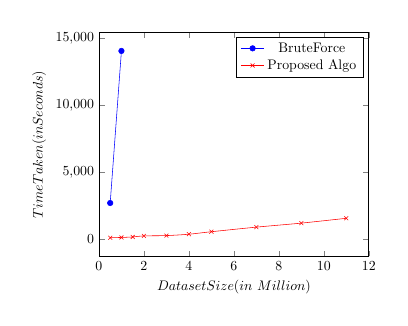
\begin{tikzpicture}[scale=0.5]
  \begin{axis}[
    xlabel=$Dataset Size(in\ Million)$,
    scaled x ticks = false,
    scaled y ticks = false,
    xmin=0, xmax=12,
    ylabel=$TimeTaken(inSeconds)$]
    \addplot[smooth,mark=*,blue] plot coordinates {
      (0.5, 2700)
      (1, 14040)
    };
    \addlegendentry{BruteForce}

    \addplot[smooth,color=red,mark=x]
    plot coordinates {
      (0.5, 108)
      (1, 132)
      (1.500, 168)
      (2.000, 246)
      (3.000, 270)
      (4.000, 372)
      (5.000, 558)
      (7.000, 900)
      (9.000, 1200)
      (11.000, 1560)
    };
    \addlegendentry{Proposed Algo}
  \end{axis}
\end{tikzpicture}

\subsection{Effect of k}

Here we have evaluated the effect of number of neighbour calculation
on the total time taken and shuffle bytes. Since the performance of bruteforce is very low, we will not using the
comparison chart anymore. Here we have used the Forest dataset with
600k vectors. The time taken increases linearly with increase in k. We
also see that the number of shuffle bytes as well increase with
increase in k. This is because with increase in k, we need to find
more k across partitions. The most of the shuffle bytes is due to
moving the results to the right node, which is unavoidable.

\medskip

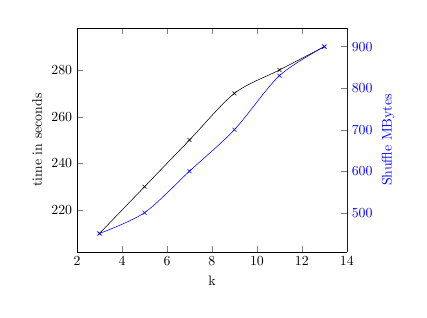
\begin{tikzpicture}[scale=0.5]
  \begin{axis}[black,
    axis y line*=left,
    xlabel=k,
    ylabel=time in seconds,
    ]
    \addplot[smooth,color=black,mark=x]
    plot coordinates {
      (3, 210)
      (5, 230)
      (7, 250)
      (9, 270)
      (11, 280)
      (13, 290)
    };
  \end{axis}

  \begin{axis}[blue,
    xlabel=k,
    ylabel=Shuffle MBytes,
    axis y line*=right,
    axis x line=none, ]
    \addplot[smooth,color=blue,mark=x]
    plot coordinates {
      (3, 450)
      (5, 500)
      (7, 600)
      (9, 700)
      (11, 830)
      (13, 900)
    };
  \end{axis}
\end{tikzpicture}

\subsection{Effect of number of pivots}
We evaluated the effect of pivots on the running time and shuffle
bytes. We found that if the number of pivots is very low the
performance is poor because then number of comparison per vector
increases. Also if the number of pivots is high, too many partition
has to be compared to find nearest neighbours. This causes number of
shuffle bytes to go high.

\medskip

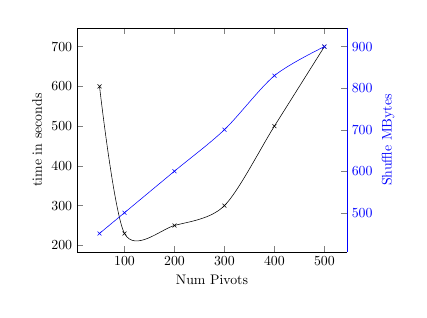
\begin{tikzpicture}[scale=0.5]
  \begin{axis}[black,
    axis y line*=left,
    xlabel=Num Pivots,
    ylabel=time in seconds,
    ]
    \addplot[smooth,color=black,mark=x]
    plot coordinates {
      (50, 600)
      (100, 230)
      (200, 250)
      (300, 300)
      (400, 500)
      (500, 700)
    };
  \end{axis}

  \begin{axis}[blue,
    xlabel=Num Pivots,
    ylabel=Shuffle MBytes,
    axis y line*=right,
    axis x line=none, ]
    \addplot[smooth,color=blue,mark=x]
    plot coordinates {
      (50, 450)
      (100, 500)
      (200, 600)
      (300, 700)
      (400, 830)
      (500, 900)
    };
  \end{axis}
\end{tikzpicture}


\subsection{Effect of dimensions}
We evaluated the increase in dimensions and found that higher the
dimensions longer the computation time. This is because at higher dimensions the distance
between closest and farthest neighbors will be nearly same
\cite{beyer_when_1999}. This also causes increase in shuffling bytes.

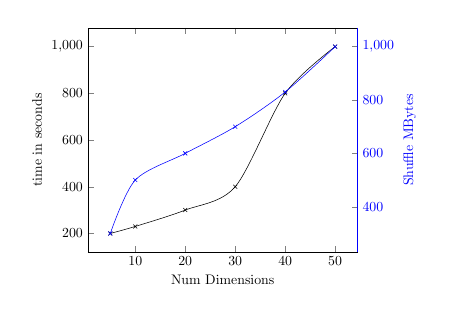
\begin{tikzpicture}[scale=0.5]
  \begin{axis}[black,
    axis y line*=left,
    xlabel=Num Dimensions,
    ylabel=time in seconds,
    ]
    \addplot[smooth,color=black,mark=x]
    plot coordinates {
      (5, 200)
      (10, 230)
      (20, 300)
      (30, 400)
      (40, 800)
      (50, 1000)
    };
  \end{axis}

  \begin{axis}[blue,
    xlabel=Num Pivots,
    ylabel=Shuffle MBytes,
    axis y line*=right,
    axis x line=none, ]
    \addplot[smooth,color=blue,mark=x]
    plot coordinates {
      (5, 300)
      (10, 500)
      (20, 600)
      (30, 700)
      (40, 830)
      (50, 1000)
    };
  \end{axis}
\end{tikzpicture}


\subsection{Effect of number of nodes}
Using distributed framework should help us achieve near linear
scalability. But once we reach a threshold the perfomance start to
remain constant because many nodes will not be used fully


\medskip

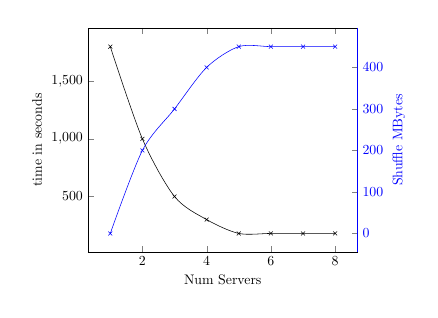
\begin{tikzpicture}[scale=0.5]
  \begin{axis}[black,
    axis y line*=left,
    xlabel=Num Servers,
    ylabel=time in seconds,
    ]
    \addplot[smooth,color=black,mark=x]
    plot coordinates {
      (1, 1800)
      (2, 1000)
      (3, 500)
      (4, 300)
      (5, 180)
      (6, 180)
      (7, 180)
      (8, 180)
    };
  \end{axis}

  \begin{axis}[blue,
    xlabel=Num Servers,
    ylabel=Shuffle MBytes,
    axis y line*=right,
    axis x line=none, ]
    \addplot[smooth,color=blue,mark=x]
    plot coordinates {
      (1, 0)
      (2, 200)
      (3, 300)
      (4, 400)
      (5, 450)
      (6, 450)
      (7, 450)
      (8, 450)
    };
  \end{axis}
\end{tikzpicture}



\bigskip

\section{Conclusion}
In this paper, we came up with an efficient algorithm KNN Join for the
distributed framework, spark. By partitioning both the dataset R and S
using voronoi based methods and finding nearest neighbour within the
same partition as only points on the edge of the partition will have
nearest neighbour in other partition. we exploited parallel processing
in spark by parallelizing computation done in each partition. The
results taken in real datasets proves that the algorithm is efficient
in both network and i/o usage and scalable.

% An example of a floating figure using the graphicx package.
% Note that \label must occur AFTER (or within) \caption.
% For figures, \caption should occur after the \includegraphics.
% Note that IEEEtran v1.7 and later has special internal code that
% is designed to preserve the operation of \label within \caption
% even when the captionsoff option is in effect. However, because
% of issues like this, it may be the safest practice to put all your
% \label just after \caption rather than within \caption{}.
%
% Reminder: the "draftcls" or "draftclsnofoot", not "draft", class
% option should be used if it is desired that the figures are to be
% displayed while in draft mode.
%
% \begin{figure}[!t]
%   \centering
%   \includegraphics[width=2.5in]{myfigure}
%   where an .eps filename suffix will be assumed under latex,
%   and a .pdf suffix will be assumed for pdflatex; or what has been declared
%   via \DeclareGraphicsExtensions.
%   \caption{Simulation results for the network.}
%   \label{fig_sim}
% \end{figure}

% Note that IEEE typically puts floats only at the top, even when this
% results in a large percentage of a column being occupied by floats.


% An example of a double column floating figure using two subfigures.
% (The subfig.sty package must be loaded for this to work.)
% The subfigure \label commands are set within each subfloat command,
% and the \label for the overall figure must come after \caption.
% \hfil is used as a separator to get equal spacing.
% Watch out that the combined width of all the subfigures on a
% line do not exceed the text width or a line break will occur.
%
% \begin{figure*}[!t]
%   \centering
%   \subfloat[Case I]{\includegraphics[width=2.5in]{box}%
%   \label{fig_first_case}}
%   \hfil
%   \subfloat[Case II]{\includegraphics[width=2.5in]{box}%
%   \label{fig_second_case}}
%   \caption{Simulation results for the network.}
%   \label{fig_sim}
% \end{figure*}
%
% Note that often IEEE papers with subfigures do not employ subfigure
% captions (using the optional argument to \subfloat[]), but instead will
% reference/describe all of them (a), (b), etc., within the main caption.
% Be aware that for subfig.sty to generate the (a), (b), etc., subfigure
% labels, the optional argument to \subfloat must be present. If a
% subcaption is not desired, just leave its contents blank,
% e.g., \subfloat[].


% An example of a floating table. Note that, for IEEE style tables, the
% \caption command should come BEFORE the table and, given that table
% captions serve much like titles, are usually capitalized except for words
% such as a, an, and, as, at, but, by, for, in, nor, of, on, or, the, to
% and up, which are usually not capitalized unless they are the first or
% last word of the caption. Table text will default to \footnotesize as
% IEEE normally uses this smaller font for tables.
% The \label must come after \caption as always.
%
% \begin{table}[!t]
%%   increase table row spacing, adjust to taste
%   \renewcommand{\arraystretch}{1.3}
%   if using array.sty, it might be a good idea to tweak the value of
%   \extrarowheight as needed to properly center the text within the cells
%   \caption{An Example of a Table}
%   \label{table_example}
%   \centering
%%   Some packages, such as MDW tools, offer better commands for making tables
%%   than the plain LaTeX2e tabular which is used here.
%   \begin{tabular}{|c||c|}
%     \hline
%     One & Two\\
%     \hline
%     Three & Four\\
%     \hline
%   \end{tabular}
% \end{table}


% Note that the IEEE does not put floats in the very first column
% - or typically anywhere on the first page for that matter. Also,
% in-text middle ("here") positioning is typically not used, but it
% is allowed and encouraged for Computer Society conferences (but
% not Computer Society journals). Most IEEE journals/conferences use
% top floats exclusively.
% Note that, LaTeX2e, unlike IEEE journals/conferences, places
% footnotes above bottom floats. This can be corrected via the
% \fnbelowfloat command of the stfloats package.

\bigskip

% trigger a \newpage just before the given reference
% number - used to balance the columns on the last page
% adjust value as needed - may need to be readjusted if
% the document is modified later
% \IEEEtriggeratref{8}
% The "triggered" command can be changed if desired:
% \IEEEtriggercmd{\enlargethispage{-5in}}

% references section
\newpage
% can use a bibliography generated by BibTeX as a .bbl file
% BibTeX documentation can be easily obtained at:
% http://www.ctan.org/tex-archive/biblio/bibtex/contrib/doc/
% The IEEEtran BibTeX style support page is at:
% http://www.michaelshell.org/tex/ieeetran/bibtex/
\bibliography{knnjoin}
\bibliographystyle{IEEEtran}
% argument is your BibTeX string definitions and bibliography database(s)

%
% <OR> manually copy in the resultant .bbl file
% set second argument of \begin to the number of references
%   (used to reserve space for the reference number labels box)
%   \begin{thebibliography}{1}

%   \bibitem{IEEEhowto:kopka}
%     H.~Kopka and P.~W. Daly, \emph{A Guide to \LaTeX}, 3rd~ed.\hskip 1em plus
%     0.5em minus 0.4em\relax Harlow, England: Addison-Wesley, 1999.

%   \end{thebibliography}




%   that's all folks
\end{document}

%%% Local Variables:
%%% mode: latex
%%% TeX-master: t
%%% End:
